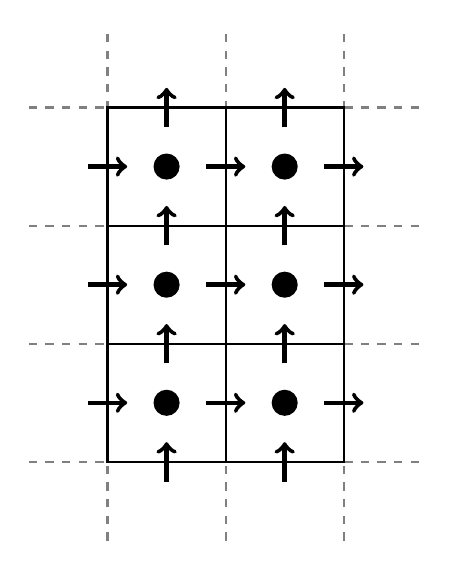
\begin{tikzpicture}

  \foreach \j in {-0.25,1.25,2.75,4.25} {
  \foreach \i in {0.75,2.25} {
    \draw[->,ultra thick] (\i,\j) -- (\i,\j+0.5){};
  } }

  \foreach \j in {0.75,2.25,3.75} {
  \foreach \i in {-0.25,1.25,2.75} {
    \draw[->,ultra thick] (\i,\j) -- (\i+0.5,\j){};
  } }

  \foreach \j in {0,1.5,3,4.5} {
    \draw[gray,thick,dashed] (-1.0,\j) -- (4.0,\j);
    }

  \foreach \i in {0,1.5,3} {
    \draw[gray,thick,dashed] (\i,-1.0) -- (\i,5.5);
    }

  \draw[thick] (0,0) rectangle (3,4.5);
  \draw[step=15mm,thick] (0,0) grid (3,4.5);

  \node at (0.75,0.75) [circle,fill=black] {};
  \node at (0.75,2.25) [circle,fill=black] {};
  \node at (0.75,3.75) [circle,fill=black] {};

  \node at (2.25,0.75) [circle,fill=black] {};
  \node at (2.25,2.25) [circle,fill=black] {};
  \node at (2.25,3.75) [circle,fill=black] {};


\end{tikzpicture}
